\documentclass[]{article}
\usepackage{lmodern}
\usepackage{amssymb,amsmath}
\usepackage{ifxetex,ifluatex}
\usepackage{fixltx2e} % provides \textsubscript
\ifnum 0\ifxetex 1\fi\ifluatex 1\fi=0 % if pdftex
  \usepackage[T1]{fontenc}
  \usepackage[utf8]{inputenc}
\else % if luatex or xelatex
  \ifxetex
    \usepackage{mathspec}
    \usepackage{xltxtra,xunicode}
  \else
    \usepackage{fontspec}
  \fi
  \defaultfontfeatures{Mapping=tex-text,Scale=MatchLowercase}
  \newcommand{\euro}{€}
    \setmainfont{Times New Roman}
\fi
% use upquote if available, for straight quotes in verbatim environments
\IfFileExists{upquote.sty}{\usepackage{upquote}}{}
% use microtype if available
\IfFileExists{microtype.sty}{%
\usepackage{microtype}
\UseMicrotypeSet[protrusion]{basicmath} % disable protrusion for tt fonts
}{}
\usepackage[margin=1in]{geometry}
\ifxetex
  \usepackage[setpagesize=false, % page size defined by xetex
              unicode=false, % unicode breaks when used with xetex
              xetex]{hyperref}
\else
  \usepackage[unicode=true]{hyperref}
\fi
\hypersetup{breaklinks=true,
            bookmarks=true,
            pdfauthor={Erich Seamon},
            pdftitle={Exploratory Data Analysis: Agricultural Commodity Loss Variations across the Pacific Northwest, narrowing to the IPNW},
            colorlinks=true,
            citecolor=blue,
            urlcolor=blue,
            linkcolor=magenta,
            pdfborder={0 0 0}}
\urlstyle{same}  % don't use monospace font for urls
\usepackage{graphicx,grffile}
\makeatletter
\def\maxwidth{\ifdim\Gin@nat@width>\linewidth\linewidth\else\Gin@nat@width\fi}
\def\maxheight{\ifdim\Gin@nat@height>\textheight\textheight\else\Gin@nat@height\fi}
\makeatother
% Scale images if necessary, so that they will not overflow the page
% margins by default, and it is still possible to overwrite the defaults
% using explicit options in \includegraphics[width, height, ...]{}
\setkeys{Gin}{width=\maxwidth,height=\maxheight,keepaspectratio}
\setlength{\parindent}{0pt}
\setlength{\parskip}{6pt plus 2pt minus 1pt}
\setlength{\emergencystretch}{3em}  % prevent overfull lines
\providecommand{\tightlist}{%
  \setlength{\itemsep}{0pt}\setlength{\parskip}{0pt}}
\setcounter{secnumdepth}{0}

%%% Use protect on footnotes to avoid problems with footnotes in titles
\let\rmarkdownfootnote\footnote%
\def\footnote{\protect\rmarkdownfootnote}

%%% Change title format to be more compact
\usepackage{titling}

% Create subtitle command for use in maketitle
\newcommand{\subtitle}[1]{
  \posttitle{
    \begin{center}\large#1\end{center}
    }
}

\setlength{\droptitle}{-2em}

  \title{Exploratory Data Analysis: Agricultural Commodity Loss Variations across
the Pacific Northwest, narrowing to the IPNW}
    \pretitle{\vspace{\droptitle}\centering\huge}
  \posttitle{\par}
    \author{Erich Seamon}
    \preauthor{\centering\large\emph}
  \postauthor{\par}
      \predate{\centering\large\emph}
  \postdate{\par}
    \date{03/01/2019}

% Redefines (sub)paragraphs to behave more like sections
\ifx\paragraph\undefined\else
\let\oldparagraph\paragraph
\renewcommand{\paragraph}[1]{\oldparagraph{#1}\mbox{}}
\fi
\ifx\subparagraph\undefined\else
\let\oldsubparagraph\subparagraph
\renewcommand{\subparagraph}[1]{\oldsubparagraph{#1}\mbox{}}
\fi

\usepackage{booktabs}
\usepackage{longtable}
\usepackage{array}
\usepackage{multirow}
\usepackage[table]{xcolor}
\usepackage{wrapfig}
\usepackage{float}
\usepackage{colortbl}
\usepackage{pdflscape}
\usepackage{tabu}
\usepackage{threeparttable}
\usepackage{threeparttablex}
\usepackage[normalem]{ulem}
\usepackage{makecell}

\begin{document}
\maketitle

\subsection{Introduction}\label{introduction}

This analysis explores the relationships of agricultural commodity loss,
at a county level, from 2001-2015, across the three state region of the
Pacific Northwest (Washington, Idaho, and Oregon), and then focusing in
on the Inland Pacific Northwest (INPW - 26 county region that
encapsulates the Palouse, in Washington, Idaho, and Oregon). Here we
explore the entire range of commodities and damage causes, identifying
the top revenue loss commodities and their most pertinent damage causes
- as indicated from the USDA's agricultural commodity loss insurance
archive. We also explore claim freqency, and finally zero in on the top
5 commodities for the region, and examine specific loss and claim
frequency by year and damage cause.

We perform several steps to examine the full set of data, and to narrow
down factors to a usable form for further modeling analysis.
\textbf{Step 1.} Data Preparation: Loading and Transforming data. Here
we load commodity loss data, and aggregate by differing factors, so we
can examine losses on an annual basis, by county, damage cause, and
commodity. \textbf{Step 2.} Study Area Overview. We narrow down our data
to the 26 county palouse region, and display a study area map for
perspective. \textbf{Step 3.} Pacific Northwest Region Overview of
Insurance Loss by year, damage cause, and commodity: 2001-2015
\textbf{Step 4.} Pacific Northwest Region Overview of Insurance Loss
FREQUENCY by commodity and damage cause: 2001-2015 \textbf{Step 5.} IPNW
Study Area Region Overview of Insurance Loss FREQUENCY by commodity and
damage cause: 2001-2015 \textbf{Step 6.} IPNW Study Area Region
Interaction Plots of Insurance Loss FREQUENCY, for WHEAT and APPLES:
2001-2015 \textbf{Step 7.} Nationwide Wheat Prices per metric ton:
2001-2015 \textbf{Step 8.} IPNW Study Area Region Overview of Insurance
Loss (\$) by Year: 1989-2015 We summarize all insurance loss by year for
1989 - 2015 - so we can then subset our analysis to a refined time
period (2001-2015). \textbf{Step 9.} IPNW Study Area Region Overview of
Insurance Loss by Commodity: 1989-2015 We summarize all commodity
insurance loss for the Palouse by commodity - so we can determine the
top insurance loss commodities for a filtered examination. \textbf{Step
10.} IPNW Study Area Region Overiew of Insurance Loss by Damage Cause:
1989-2015. Similarly to Step 3, we summarize all insurance loss by the
cause of the damage for 1989 - 2015, so we can determine which damage
causes are resulting the the majority of insurance loss. \textbf{Step
11.} IPNW Study Area Region Overview of Insurance Loss by Commodity:
2001 - 2015. Given our previous steps, we now examine Palouse commodity
insurance loss for 2001 - 2015. \textbf{Step 12.} IPNW Study Area Region
Overiew of Insurance Loss by Damage Cause: 2001-2015. In step 8, we
examine Palouse commodities by damage cause for 2001-2015. \textbf{Step
13.} Top five commodities, 2001-2015 for the IPNW Region Study Area. In
step 13, we examine the IPNW top five commodities for 2001-2015 (apples,
wheat, cherries, dry peas, and barley).

\subsection{Step 1. Data Preparation: Loading and Transformation
data}\label{step-1.-data-preparation-loading-and-transformation-data}

The first step is to load Pacific Northwest agricultural insurance
commodity loss data, aggregate by county, damage cause and commodity,
remove zeros, transform the loss values (\$) into cube root and
logrithmic outputs, and scale and center the data.

\subsection{Step 2: Study Area Overview - 26 County Palouse
Region}\label{step-2-study-area-overview---26-county-palouse-region}

\begin{verbatim}
## Error in match.fun(FUN): object 'HTML' not found
\end{verbatim}

\begin{verbatim}
## Error in getMapData(map): object 'map' not found
\end{verbatim}

\begin{verbatim}
## $interactive
## [1] TRUE
## 
## $draggable
## [1] FALSE
## 
## $keyboard
## [1] TRUE
## 
## $title
## [1] ""
## 
## $alt
## [1] ""
## 
## $zIndexOffset
## [1] 0
## 
## $opacity
## [1] 1
## 
## $riseOnHover
## [1] TRUE
## 
## $riseOffset
## [1] 250
\end{verbatim}

/

\subsection{Step 3: Pacific Northwest Region Overview of Insurance Loss
by year, damage cause, and commodity:
2001-2015}\label{step-3-pacific-northwest-region-overview-of-insurance-loss-by-year-damage-cause-and-commodity-2001-2015}

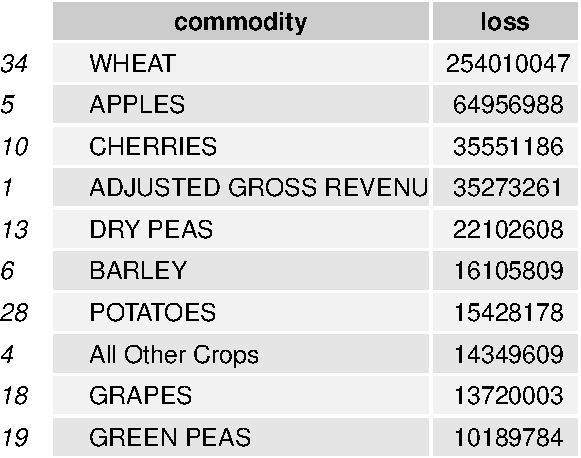
\includegraphics{dmine-mixedmodel-analysis_Phase1_files/figure-latex/unnamed-chunk-3-1.pdf}

PNW total insurance loss by year, 2001-2015

2001-2015

damage cause

loss

Drought

\$719,610,396

Decline in Price

\$336,993,981

Heat

\$267,376,106

Frost

\$170,482,583

Freeze

\$149,373,220

Excess Moisture/Precip/Rain

\$148,556,853

Hail

\$127,772,100

Cold Wet Weather

\$86,741,055

Cold Winter

\$67,118,523

Failure Irrig Supply

\$57,087,916

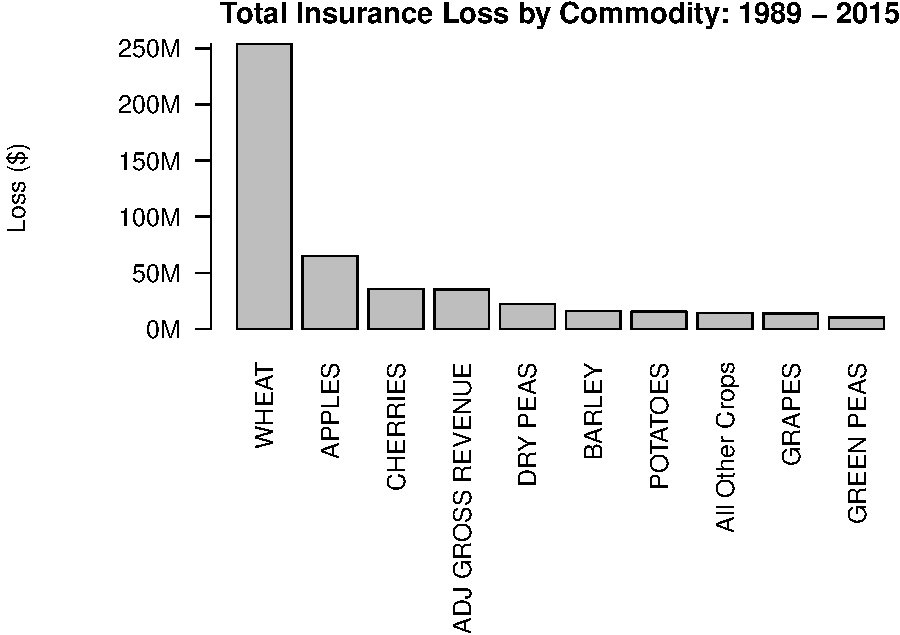
\includegraphics{dmine-mixedmodel-analysis_Phase1_files/figure-latex/unnamed-chunk-3-2.pdf}

PNW total insurance loss by year, 2001-2015

2001-2015

commodity

loss

WHEAT

\$1,444,149,995

CHERRIES

\$156,670,513

APPLES

\$156,063,380

POTATOES

\$117,459,400

BARLEY

\$102,125,046

DRY PEAS

\$58,038,162

\includegraphics{dmine-mixedmodel-analysis_Phase1_files/figure-latex/unnamed-chunk-3-3.pdf}

PNW total insurance loss by year, 2001-2015

2001-2015

year

loss

2001

\$66,499,267

2002

\$96,367,644

2003

\$103,553,264

2004

\$52,006,242

2005

\$72,871,250

2006

\$63,467,130

2007

\$83,252,301

2008

\$150,480,619

2009

\$545,650,029

2010

\$83,829,994

2011

\$115,965,036

2012

\$89,684,692

2013

\$171,121,810

2014

\$222,526,098

2015

\$296,416,750

\subsection{Step 4: Pacific Northwest Region Overview of Insurance Loss
FREQUENCY by commodity and damage cause:
2001-2015}\label{step-4-pacific-northwest-region-overview-of-insurance-loss-frequency-by-commodity-and-damage-cause-2001-2015}

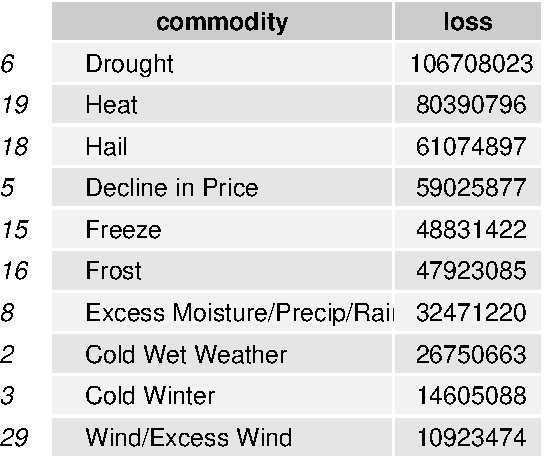
\includegraphics{dmine-mixedmodel-analysis_Phase1_files/figure-latex/unnamed-chunk-4-1.pdf}
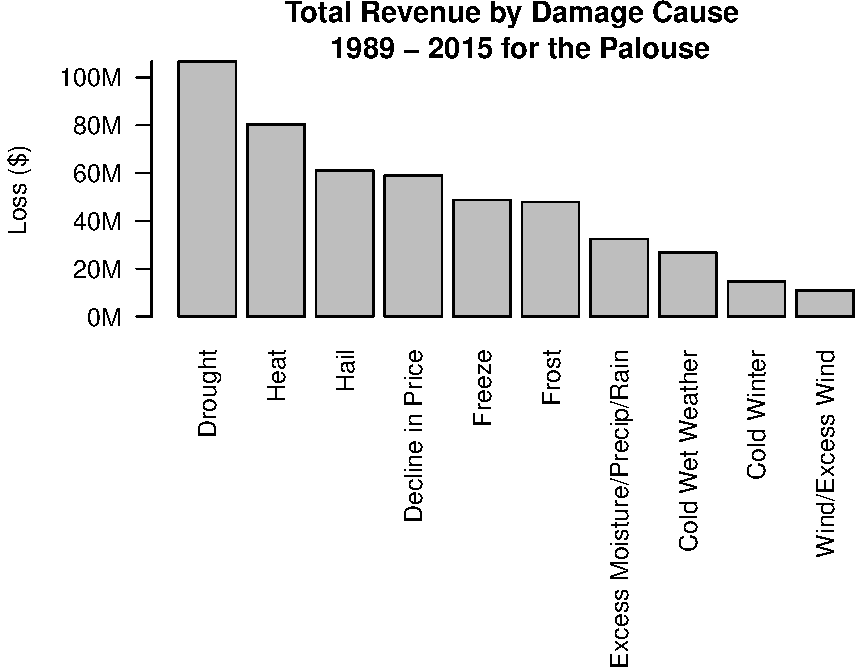
\includegraphics{dmine-mixedmodel-analysis_Phase1_files/figure-latex/unnamed-chunk-4-2.pdf}

/

\subsection{Step 5: IPNW Study Area Region Overview of Insurance Loss
FREQUENCY by commodity and damage cause:
2001-2015}\label{step-5-ipnw-study-area-region-overview-of-insurance-loss-frequency-by-commodity-and-damage-cause-2001-2015}

\includegraphics{dmine-mixedmodel-analysis_Phase1_files/figure-latex/unnamed-chunk-5-1.pdf}
\includegraphics{dmine-mixedmodel-analysis_Phase1_files/figure-latex/unnamed-chunk-5-2.pdf}
/

\subsection{Step 6: IPNW Study Area Region Interaction Plots of
Insurance Loss FREQUENCY, for WHEAT and APPLES:
2001-2015}\label{step-6-ipnw-study-area-region-interaction-plots-of-insurance-loss-frequency-for-wheat-and-apples-2001-2015}

\includegraphics{dmine-mixedmodel-analysis_Phase1_files/figure-latex/unnamed-chunk-6-1.pdf}
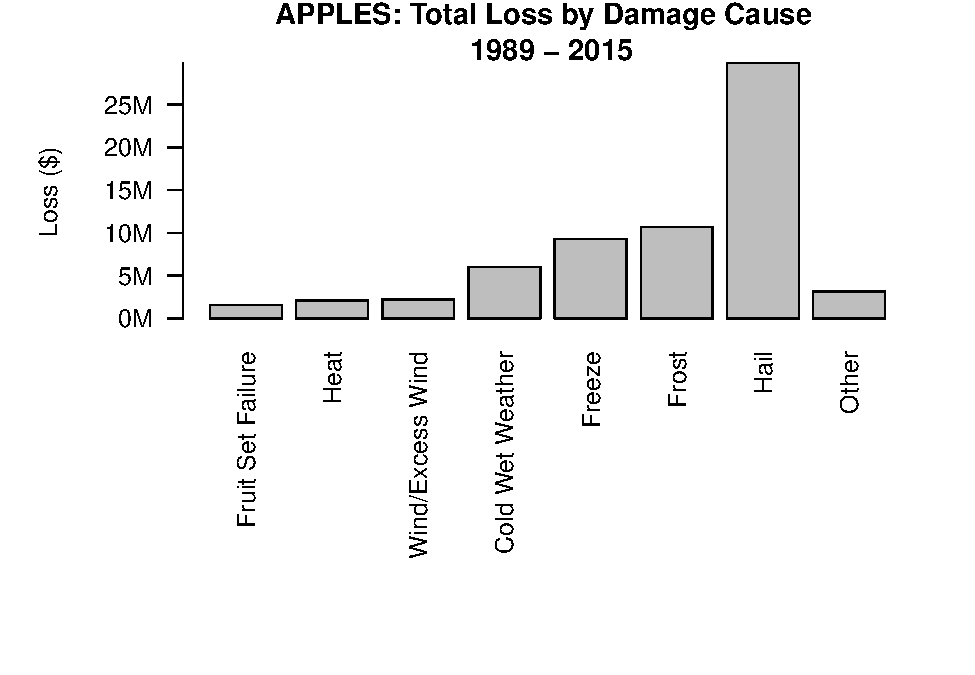
\includegraphics{dmine-mixedmodel-analysis_Phase1_files/figure-latex/unnamed-chunk-6-2.pdf}

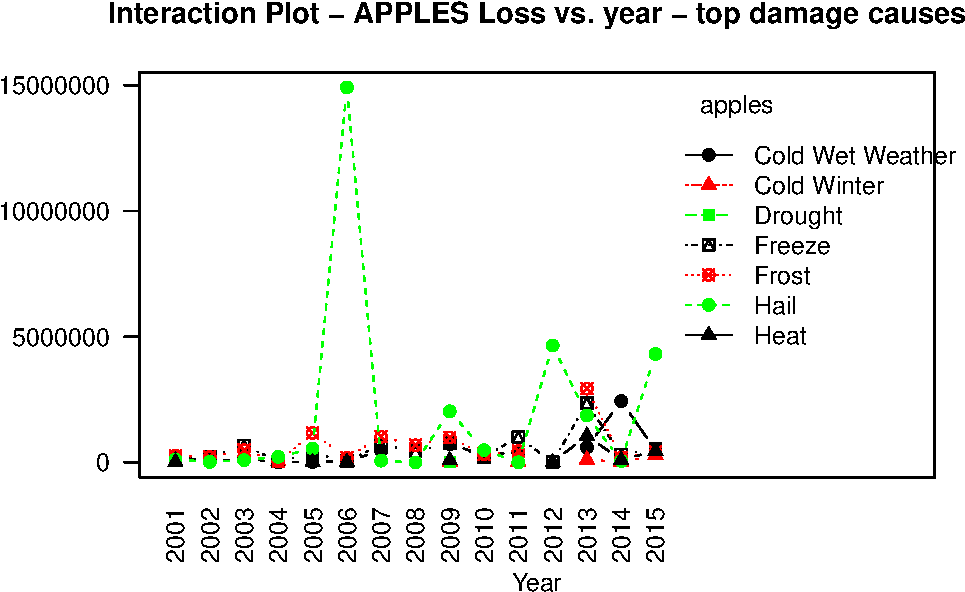
\includegraphics{dmine-mixedmodel-analysis_Phase1_files/figure-latex/unnamed-chunk-7-1.pdf}
\includegraphics{dmine-mixedmodel-analysis_Phase1_files/figure-latex/unnamed-chunk-7-2.pdf}

/

\subsection{Step 7: Nationwide Wheat Prices per metric ton:
2001-2015}\label{step-7-nationwide-wheat-prices-per-metric-ton-2001-2015}

\includegraphics{dmine-mixedmodel-analysis_Phase1_files/figure-latex/unnamed-chunk-8-1.pdf}

/

\subsection{Step 8: IPNW Study Area Region Overview of Insurance Loss
(\$) by Year:
1989-2015}\label{step-8-ipnw-study-area-region-overview-of-insurance-loss-by-year-1989-2015}

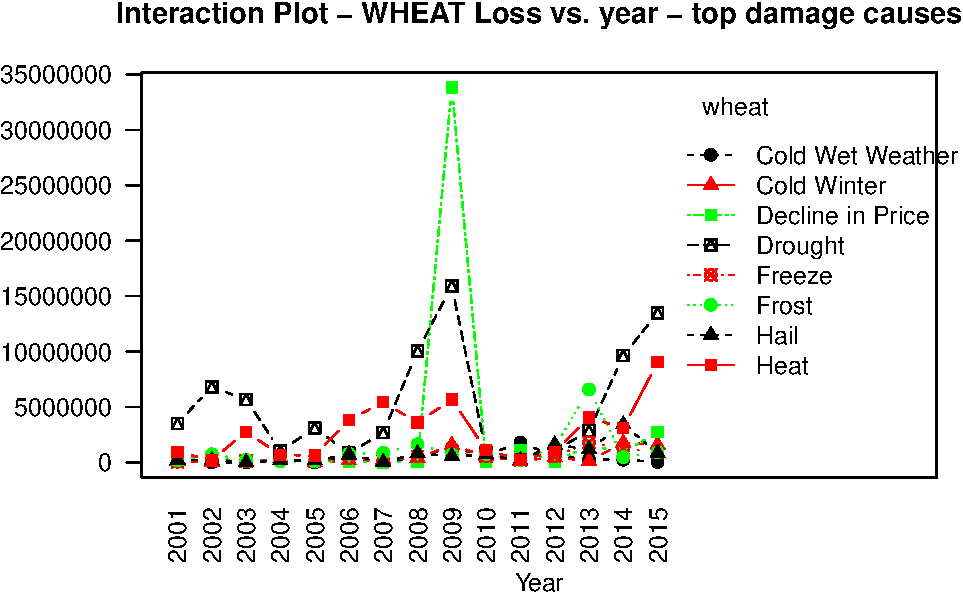
\includegraphics{dmine-mixedmodel-analysis_Phase1_files/figure-latex/unnamed-chunk-9-1.pdf}

IPNW region total insurance loss by year, 2001-2015

2001-2015

year

loss

1989

\$14,383,209

1990

\$10,730,630

1991

\$19,316,100

1992

\$22,605,598

1993

\$3,445,573

1994

\$6,712,202

1995

\$7,971,620

1996

\$8,637,903

1997

\$4,971,506

1998

\$8,899,691

1999

\$35,958,485

2000

\$28,466,133

2001

\$51,669,997

2002

\$75,193,597

2003

\$71,122,910

\subsection{Step 9: IPNW Study Area Region Overview of Insurance Loss by
Commodity:
2001-2015}\label{step-9-ipnw-study-area-region-overview-of-insurance-loss-by-commodity-2001-2015}

\includegraphics{dmine-mixedmodel-analysis_Phase1_files/figure-latex/unnamed-chunk-10-1.pdf}

IPNW region total insurance loss by commodity, 2001-2015

2001-2015

commodity

loss

WHEAT

\$1,317,798,273

APPLES

\$100,107,372

CHERRIES

\$76,366,098

DRY PEAS

\$61,746,537

BARLEY

\$39,688,619

All Other Crops

\$27,584,951

GRAPES

\$23,377,711

POTATOES

\$21,125,554

GREEN PEAS

\$16,051,658

CANOLA

\$11,643,733

ADJUSTED GROSS REVENUE-LITE

\$8,128,725

\subsection{STEP 10: IPNW Study Area Region Overiew of Insurance Loss by
Damage Cause:
2001-2015}\label{step-10-ipnw-study-area-region-overiew-of-insurance-loss-by-damage-cause-2001-2015}

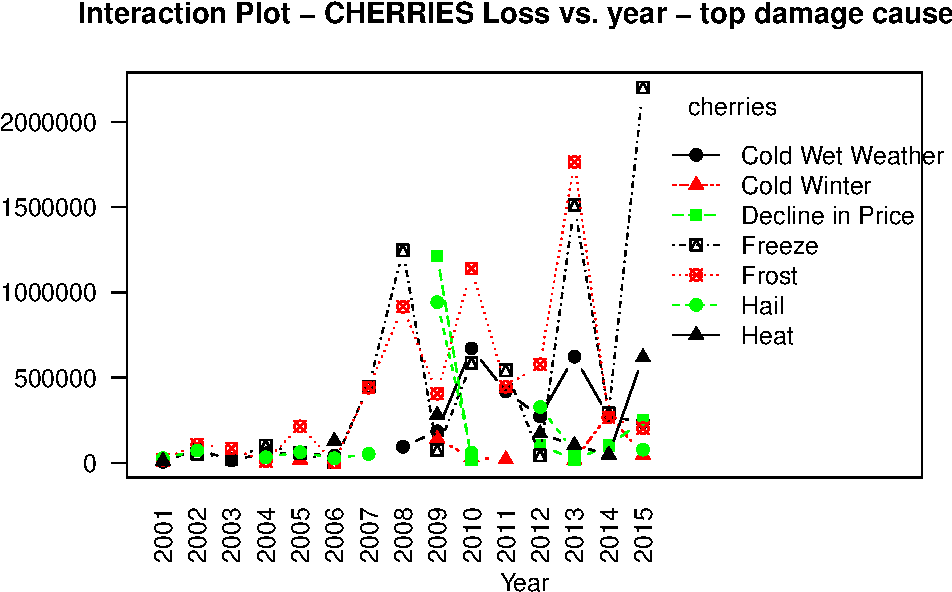
\includegraphics{dmine-mixedmodel-analysis_Phase1_files/figure-latex/unnamed-chunk-11-1.pdf}

IPNW region total insurance loss by damage cause, 2001-2015

2001-2015

damage cause

loss

Drought

\$758,075,864

Decline in Price

\$294,965,463

Heat

\$212,450,870

Frost

\$102,859,510

Freeze

\$99,682,240

Hail

\$89,981,626

Excessive Moisture

\$82,421,486

Cold Wet Weather

\$60,504,756

Cold Winter

\$39,631,809

Wind/Excess Wind

\$15,239,474

\subsection{Step 11: IPNW Study Area Region Overview of Insurance Loss
by Commodity: 2001 -
2015}\label{step-11-ipnw-study-area-region-overview-of-insurance-loss-by-commodity-2001---2015}

\includegraphics{dmine-mixedmodel-analysis_Phase1_files/figure-latex/unnamed-chunk-12-1.pdf}

IPNW region total insurance loss by commodity, 2001-2015

2001-2015

commodity

loss

WHEAT

\$1,214,345,016

APPLES

\$89,191,032

CHERRIES

\$74,853,794

DRY PEAS

\$56,809,377

BARLEY

\$34,102,839

GRAPES

\$17,370,434

GREEN PEAS

\$13,520,586

POTATOES

\$10,232,481

All Other Crops

\$9,767,559

CANOLA

\$8,913,093

ADJUSTED GROSS REVENUE-LITE

\$8,128,725

\subsection{STEP 12: IPNW Study Area Region Overiew of Insurance Loss by
Damage Cause:
2001-2015}\label{step-12-ipnw-study-area-region-overiew-of-insurance-loss-by-damage-cause-2001-2015}

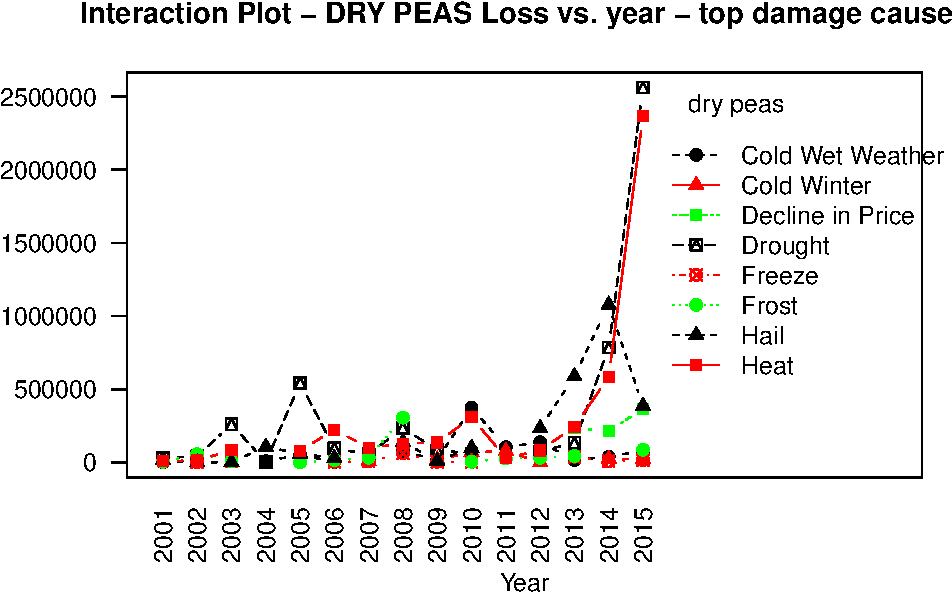
\includegraphics{dmine-mixedmodel-analysis_Phase1_files/figure-latex/unnamed-chunk-13-1.pdf}

IPNW region total insurance loss by damage cause, 2001-2015

2001-2015

commodity

loss

Drought

\$677,383,459

Decline in Price

\$290,497,980

Heat

\$197,657,025

Frost

\$92,483,544

Hail

\$81,461,121

Freeze

\$77,583,017

Excessive Moisture

\$76,603,640

Cold Wet Weather

\$54,410,357

Cold Winter

\$33,893,991

Wind/Excess Wind

\$12,442,392

\subsection{STEP 13: Top five commodities, 2001-2015 for the IPNW Region
Study
Area}\label{step-13-top-five-commodities-2001-2015-for-the-ipnw-region-study-area}

\subsubsection{Top Damage Causes for APPLES, 2001-2015 for the Palouse
Region}\label{top-damage-causes-for-apples-2001-2015-for-the-palouse-region}

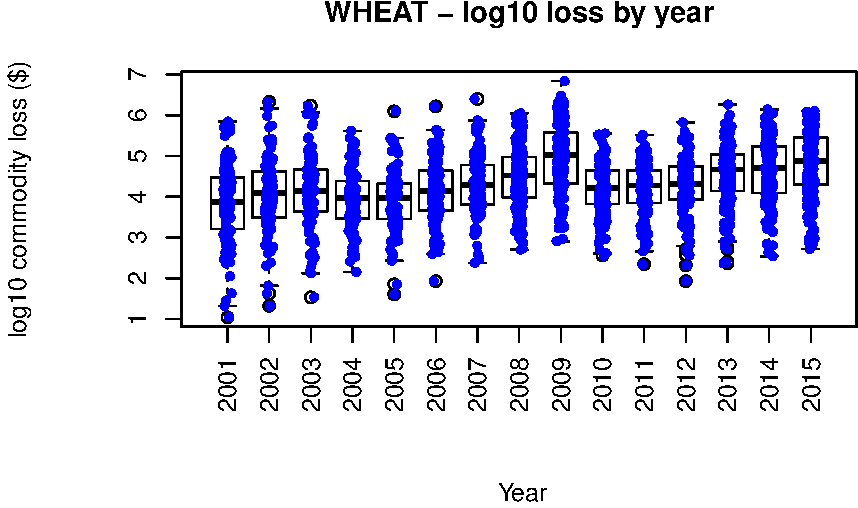
\includegraphics{dmine-mixedmodel-analysis_Phase1_files/figure-latex/unnamed-chunk-15-1.pdf}

IPNW region APPLES total insurance loss by damage cause, 2001-2015

2001-2015

damagecause

loss

Hail

\$40,971,994

Frost

\$17,016,586

Freeze

\$14,538,852

Cold Wet Weather

\$9,246,848

Wind/Excess Wind

\$2,934,044

Heat

\$2,422,480

Other

\$2,060,230

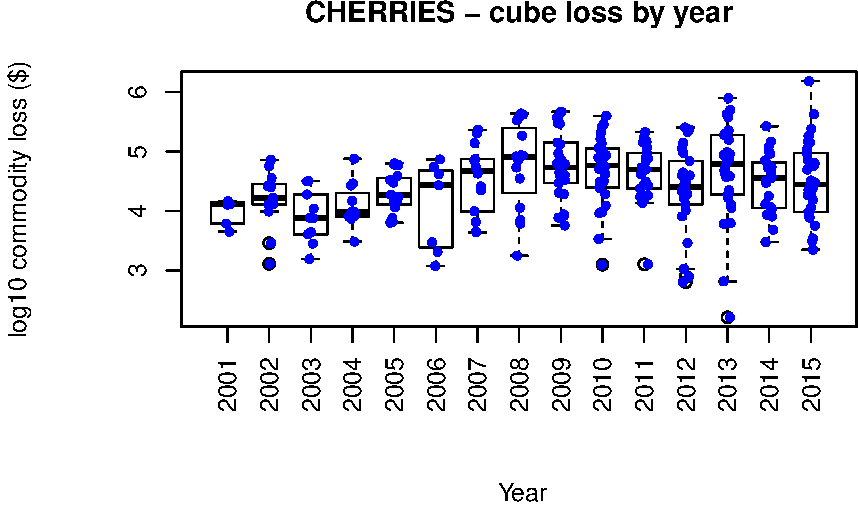
\includegraphics{dmine-mixedmodel-analysis_Phase1_files/figure-latex/unnamed-chunk-16-1.pdf}
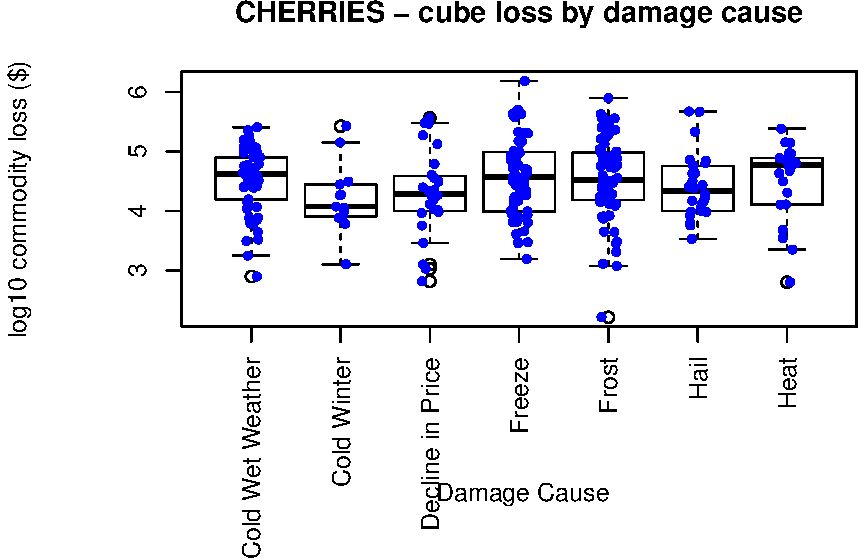
\includegraphics{dmine-mixedmodel-analysis_Phase1_files/figure-latex/unnamed-chunk-16-2.pdf}
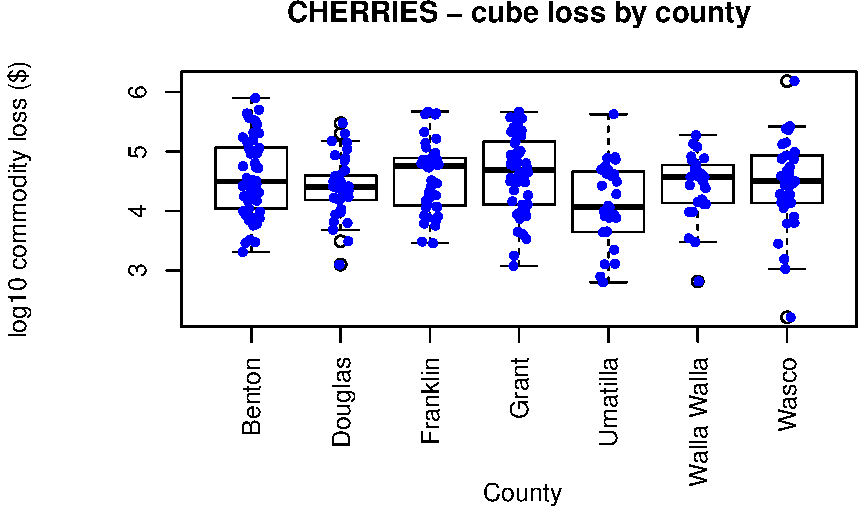
\includegraphics{dmine-mixedmodel-analysis_Phase1_files/figure-latex/unnamed-chunk-16-3.pdf}
\includegraphics{dmine-mixedmodel-analysis_Phase1_files/figure-latex/unnamed-chunk-16-4.pdf}

\begin{verbatim}
## Error in match.fun(FUN): object 'HTML' not found
\end{verbatim}

\begin{verbatim}
## Error in getMapData(map): object 'map' not found
\end{verbatim}

\begin{verbatim}
## $interactive
## [1] TRUE
## 
## $draggable
## [1] FALSE
## 
## $keyboard
## [1] TRUE
## 
## $title
## [1] ""
## 
## $alt
## [1] ""
## 
## $zIndexOffset
## [1] 0
## 
## $opacity
## [1] 1
## 
## $riseOnHover
## [1] TRUE
## 
## $riseOffset
## [1] 250
\end{verbatim}

\subsubsection{Top Damage Causes for BARLEY, 2001-2015 for the Palouse
Region}\label{top-damage-causes-for-barley-2001-2015-for-the-palouse-region}

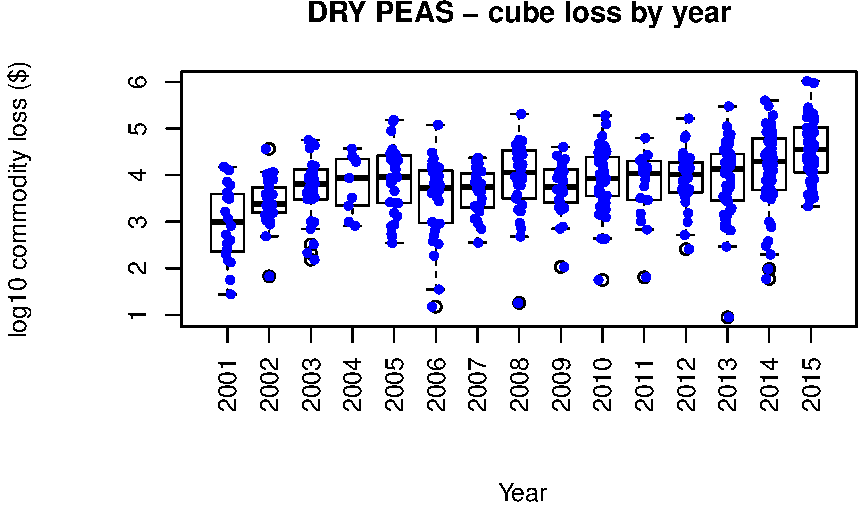
\includegraphics{dmine-mixedmodel-analysis_Phase1_files/figure-latex/unnamed-chunk-17-1.pdf}

IPNW region BARLEY total insurance loss by damage cause, 2001-2015

2001-2015

damagecause

loss

Drought

\$19,635,980

Excess Moisture/Precip/Rain

\$4,726,399

Heat

\$4,553,252

Hail

\$1,466,219

Frost

\$1,247,180

Other

\$1,085,647

Decline in Price

\$858,459

Cold Wet Weather

\$529,703

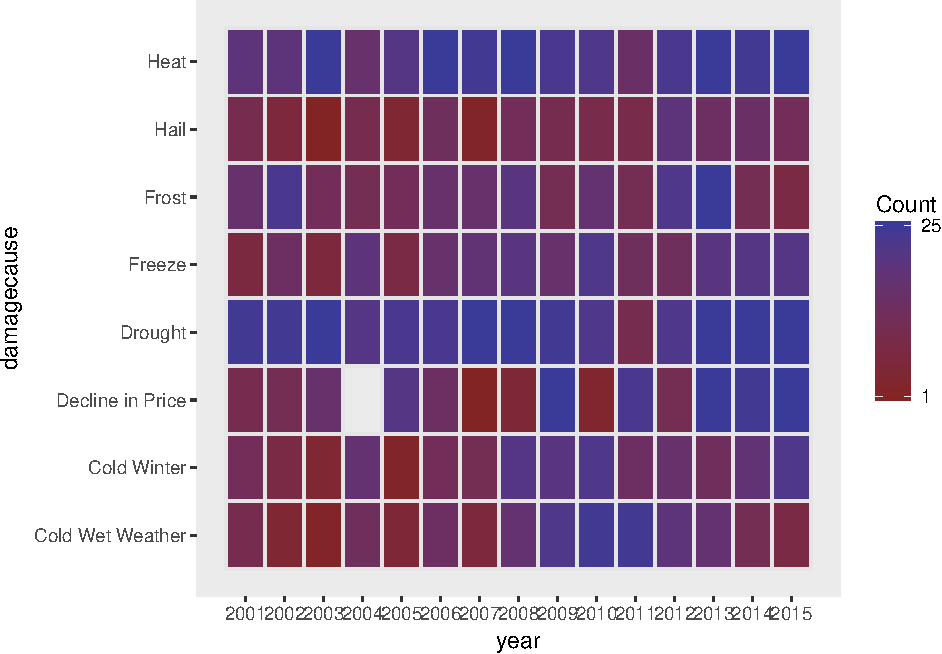
\includegraphics{dmine-mixedmodel-analysis_Phase1_files/figure-latex/unnamed-chunk-18-1.pdf}
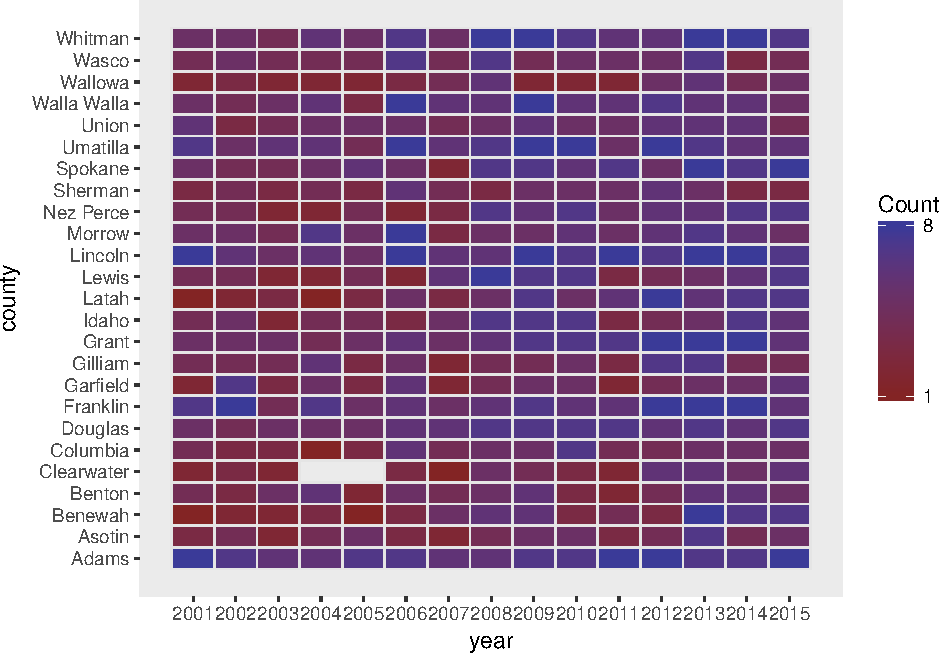
\includegraphics{dmine-mixedmodel-analysis_Phase1_files/figure-latex/unnamed-chunk-18-2.pdf}
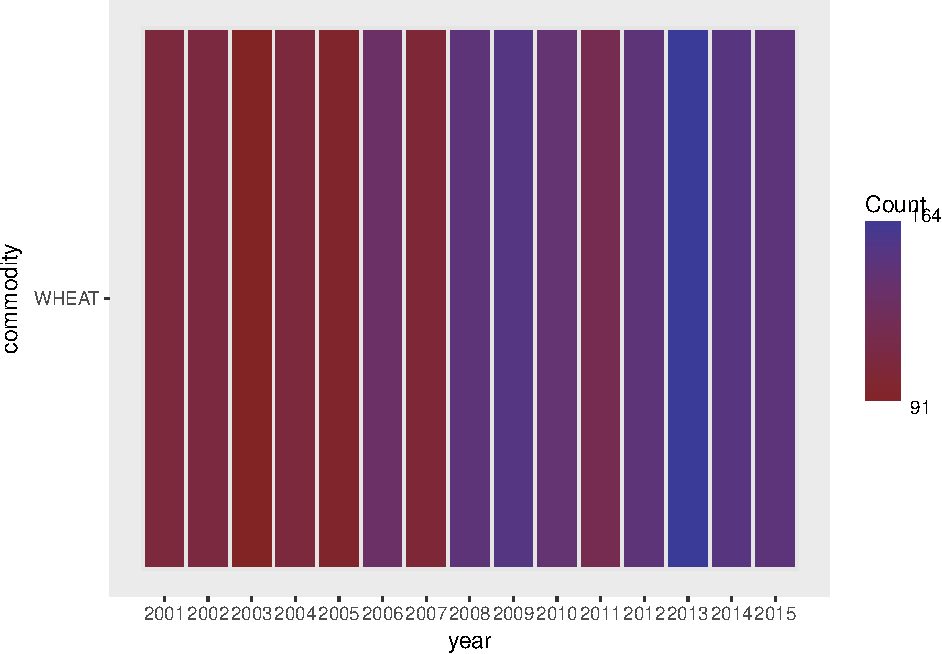
\includegraphics{dmine-mixedmodel-analysis_Phase1_files/figure-latex/unnamed-chunk-18-3.pdf}
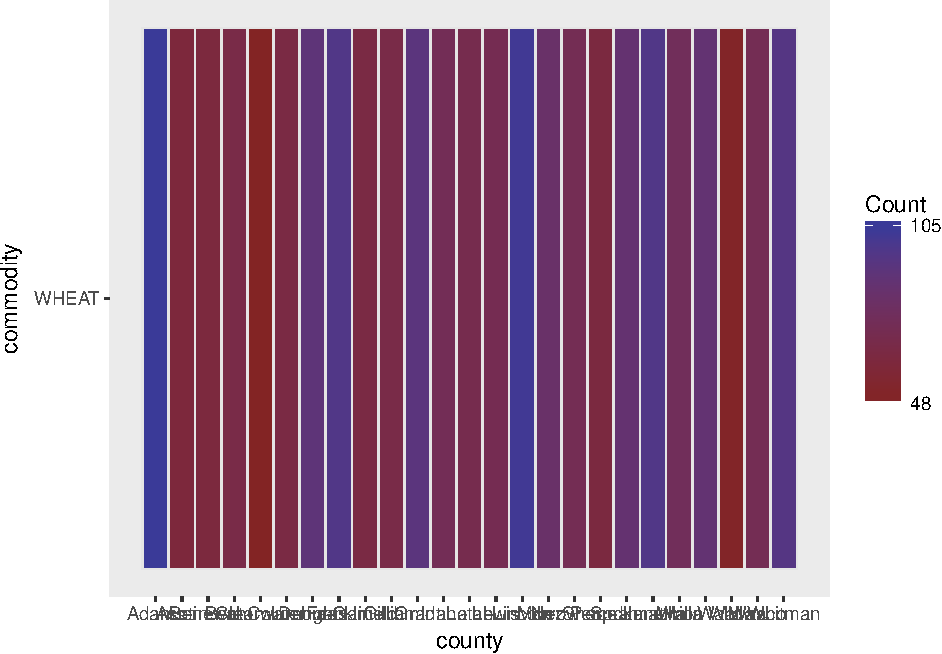
\includegraphics{dmine-mixedmodel-analysis_Phase1_files/figure-latex/unnamed-chunk-18-4.pdf}

\begin{verbatim}
## Error in brewer.pal(11, "YlOrRd"): could not find function "brewer.pal"
\end{verbatim}

\begin{verbatim}
## Error in pal(county_barley_droughtheat$loss): could not find function "pal"
\end{verbatim}

\begin{verbatim}
## Error in getMapData(map): object 'map' not found
\end{verbatim}

\begin{verbatim}
## $interactive
## [1] TRUE
## 
## $draggable
## [1] FALSE
## 
## $keyboard
## [1] TRUE
## 
## $title
## [1] ""
## 
## $alt
## [1] ""
## 
## $zIndexOffset
## [1] 0
## 
## $opacity
## [1] 1
## 
## $riseOnHover
## [1] TRUE
## 
## $riseOffset
## [1] 250
\end{verbatim}

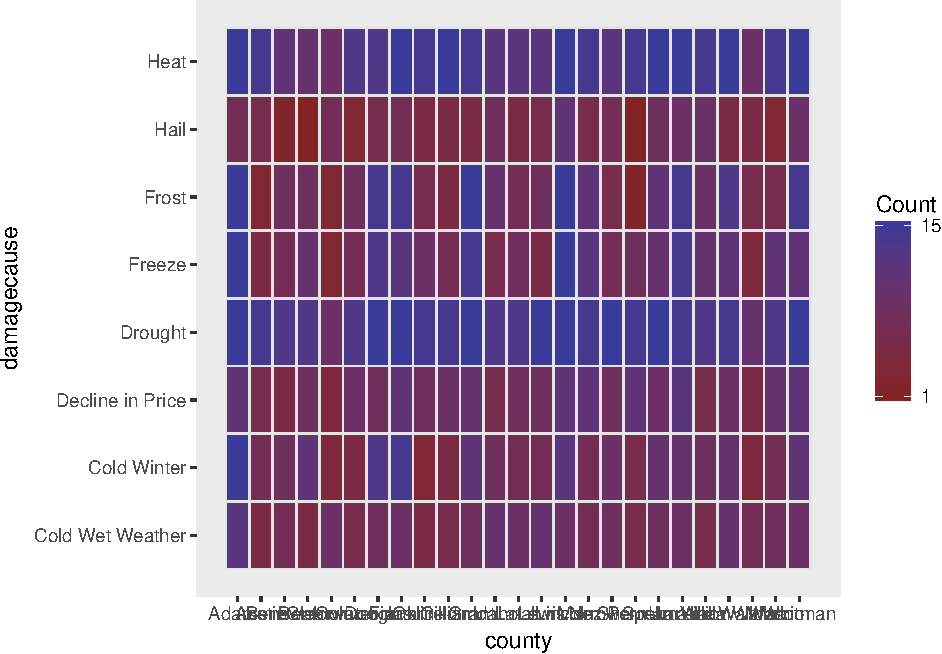
\includegraphics{dmine-mixedmodel-analysis_Phase1_files/figure-latex/unnamed-chunk-18-5.pdf}
/

\subsubsection{Top Damage Causes for WHEAT, 2001-2015 for the Palouse
Region}\label{top-damage-causes-for-wheat-2001-2015-for-the-palouse-region}

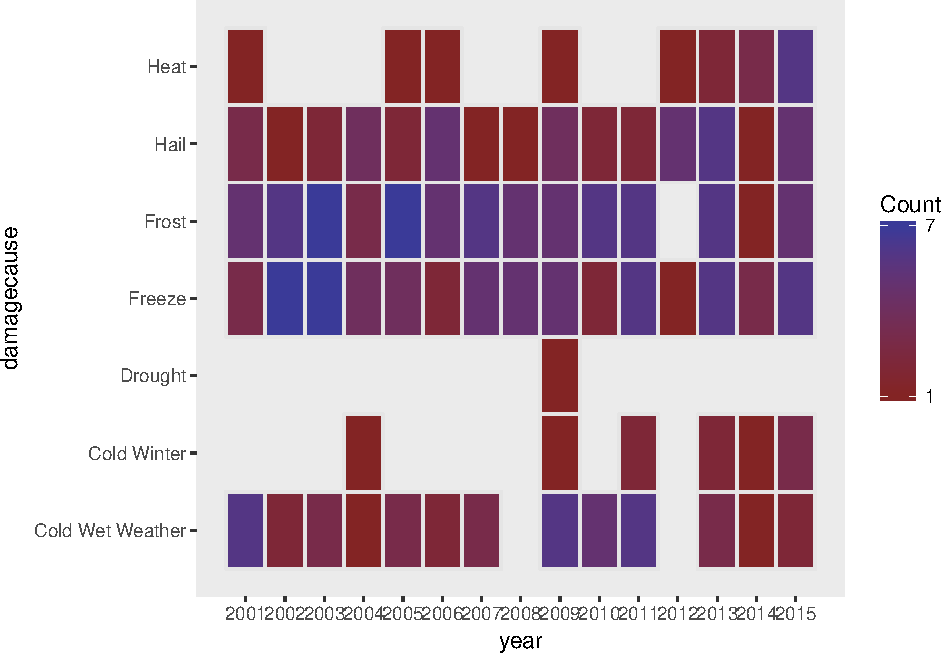
\includegraphics{dmine-mixedmodel-analysis_Phase1_files/figure-latex/unnamed-chunk-19-1.pdf}

IPNW region WHEAT total insurance loss by damage cause, 2001-2015

2001-2015

damagecause

loss

Drought

\$626,038,990

Decline in Price

\$243,681,710

Heat

\$150,761,018

Frost

\$45,605,476

Excess Moisture/Precip/Rain

\$33,421,663

Cold Winter

\$28,004,014

Freeze

\$27,203,439

Cold Wet Weather

\$24,511,419

Hail

\$20,390,532

Other

\$9,724,032

Plant Disease

\$2,950,763

Other (Snow-Lightning-Etc.)

\$2,051,960

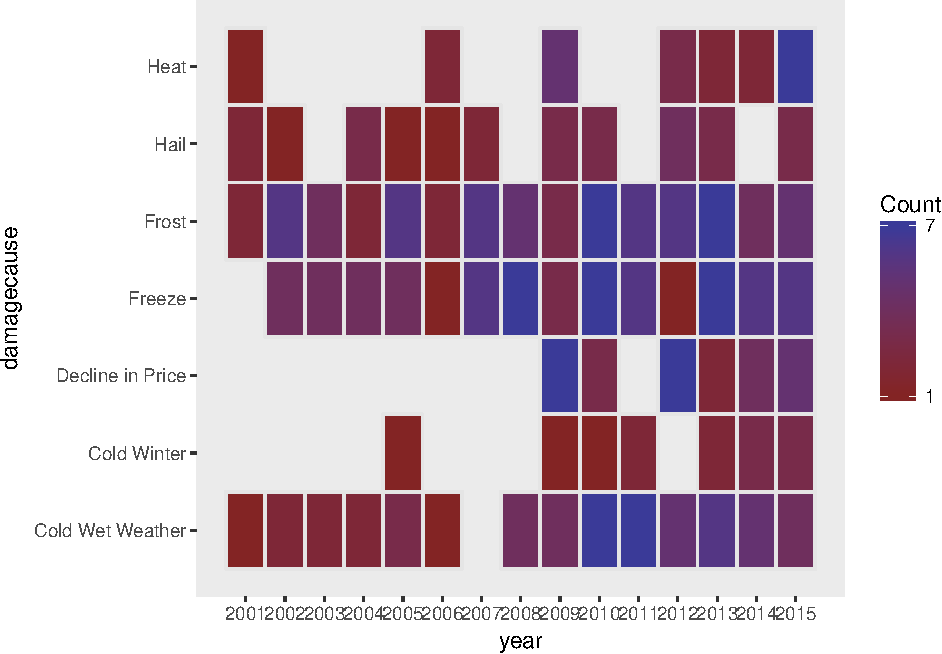
\includegraphics{dmine-mixedmodel-analysis_Phase1_files/figure-latex/unnamed-chunk-20-1.pdf}
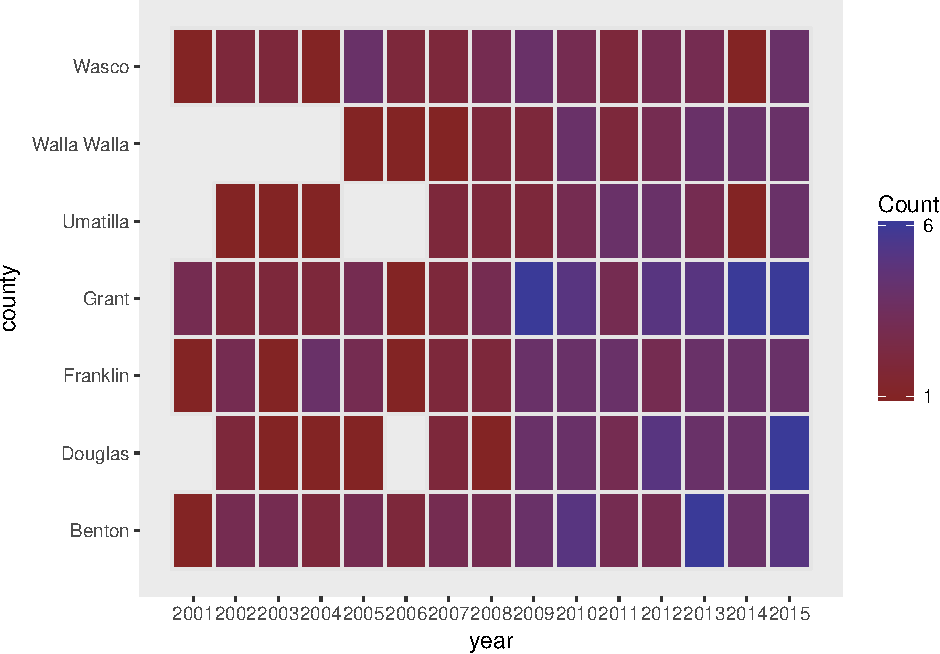
\includegraphics{dmine-mixedmodel-analysis_Phase1_files/figure-latex/unnamed-chunk-20-2.pdf}
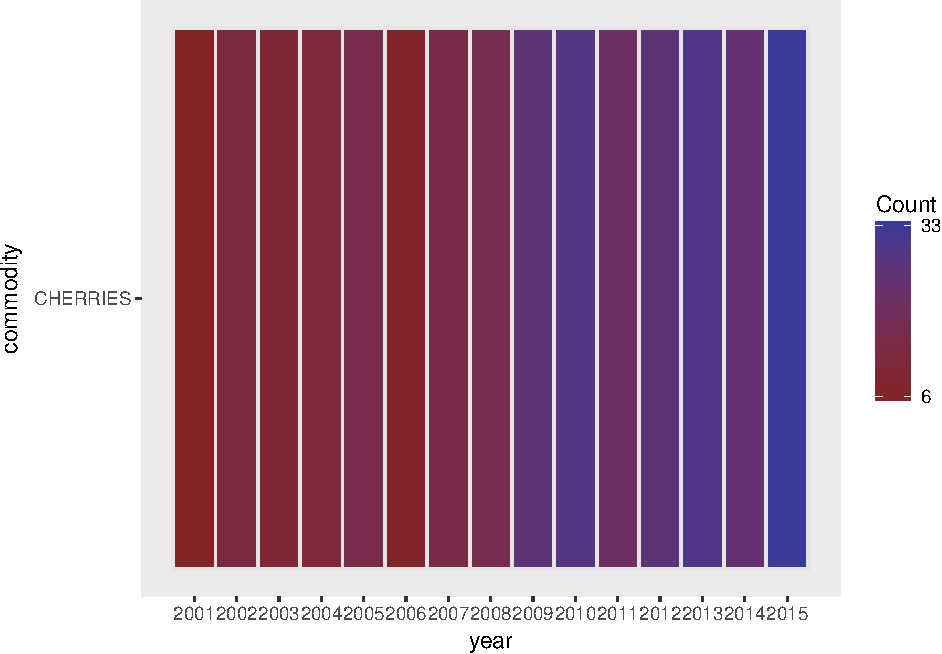
\includegraphics{dmine-mixedmodel-analysis_Phase1_files/figure-latex/unnamed-chunk-20-3.pdf}
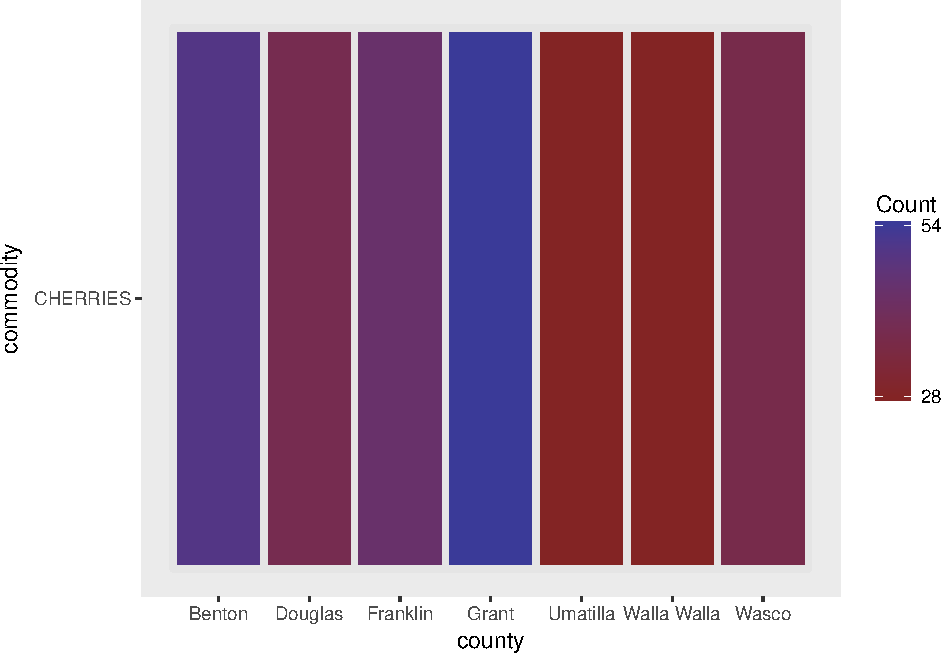
\includegraphics{dmine-mixedmodel-analysis_Phase1_files/figure-latex/unnamed-chunk-20-4.pdf}

\begin{verbatim}
## Error in brewer.pal(11, "YlOrRd"): could not find function "brewer.pal"
\end{verbatim}

\begin{verbatim}
## Error in pal(county_wheat_droughtheat$loss): could not find function "pal"
\end{verbatim}

\begin{verbatim}
## Error in getMapData(map): object 'map' not found
\end{verbatim}

\begin{verbatim}
## $interactive
## [1] TRUE
## 
## $draggable
## [1] FALSE
## 
## $keyboard
## [1] TRUE
## 
## $title
## [1] ""
## 
## $alt
## [1] ""
## 
## $zIndexOffset
## [1] 0
## 
## $opacity
## [1] 1
## 
## $riseOnHover
## [1] TRUE
## 
## $riseOffset
## [1] 250
\end{verbatim}

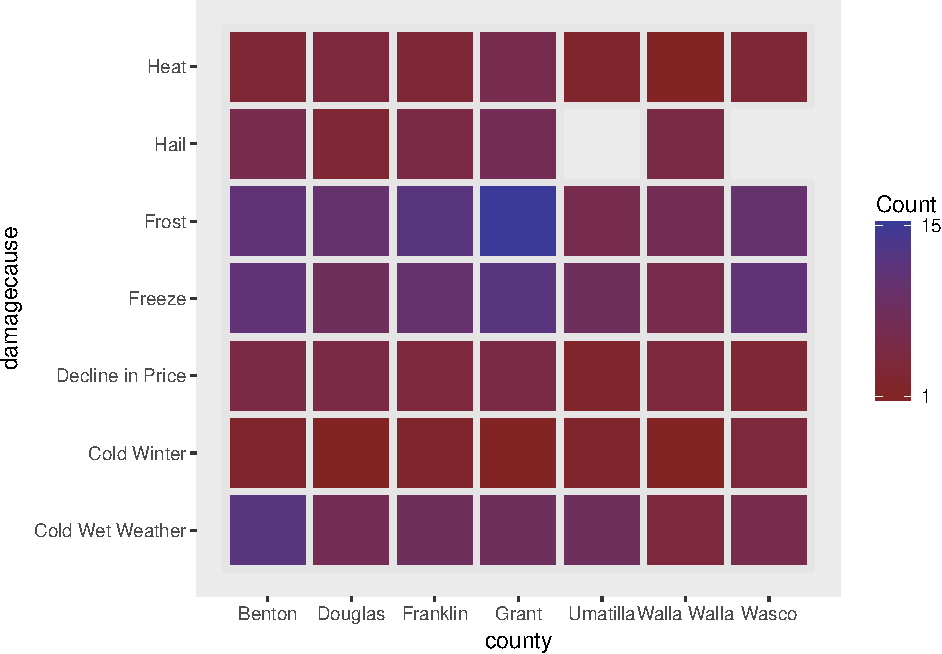
\includegraphics{dmine-mixedmodel-analysis_Phase1_files/figure-latex/unnamed-chunk-20-5.pdf}

\begin{verbatim}
## Error in brewer.pal(11, "YlOrRd"): could not find function "brewer.pal"
\end{verbatim}

\begin{verbatim}
## Error in pal(county_wheat_droughtheat2011$loss): could not find function "pal"
\end{verbatim}

\begin{verbatim}
## Error in getMapData(map): object 'map' not found
\end{verbatim}

\begin{verbatim}
## $interactive
## [1] TRUE
## 
## $draggable
## [1] FALSE
## 
## $keyboard
## [1] TRUE
## 
## $title
## [1] ""
## 
## $alt
## [1] ""
## 
## $zIndexOffset
## [1] 0
## 
## $opacity
## [1] 1
## 
## $riseOnHover
## [1] TRUE
## 
## $riseOffset
## [1] 250
\end{verbatim}

\includegraphics{dmine-mixedmodel-analysis_Phase1_files/figure-latex/unnamed-chunk-20-6.pdf}

\begin{verbatim}
## Error in brewer.pal(11, "YlOrRd"): could not find function "brewer.pal"
\end{verbatim}

\begin{verbatim}
## Error in pal(county_wheat_droughtheat2009$loss): could not find function "pal"
\end{verbatim}

\begin{verbatim}
## Error in getMapData(map): object 'map' not found
\end{verbatim}

\begin{verbatim}
## $interactive
## [1] TRUE
## 
## $draggable
## [1] FALSE
## 
## $keyboard
## [1] TRUE
## 
## $title
## [1] ""
## 
## $alt
## [1] ""
## 
## $zIndexOffset
## [1] 0
## 
## $opacity
## [1] 1
## 
## $riseOnHover
## [1] TRUE
## 
## $riseOffset
## [1] 250
\end{verbatim}

\includegraphics{dmine-mixedmodel-analysis_Phase1_files/figure-latex/unnamed-chunk-20-7.pdf}

\begin{verbatim}
## Error in brewer.pal(11, "YlOrRd"): could not find function "brewer.pal"
\end{verbatim}

\begin{verbatim}
## Error in pal(county_wheat_droughtheat2015$loss): could not find function "pal"
\end{verbatim}

\begin{verbatim}
## Error in getMapData(map): object 'map' not found
\end{verbatim}

\begin{verbatim}
## $interactive
## [1] TRUE
## 
## $draggable
## [1] FALSE
## 
## $keyboard
## [1] TRUE
## 
## $title
## [1] ""
## 
## $alt
## [1] ""
## 
## $zIndexOffset
## [1] 0
## 
## $opacity
## [1] 1
## 
## $riseOnHover
## [1] TRUE
## 
## $riseOffset
## [1] 250
\end{verbatim}

\includegraphics{dmine-mixedmodel-analysis_Phase1_files/figure-latex/unnamed-chunk-20-8.pdf}
/

\subsubsection{Top Damage Causes for CHERRIES, 2001-2015 for the Palouse
Region}\label{top-damage-causes-for-cherries-2001-2015-for-the-palouse-region}

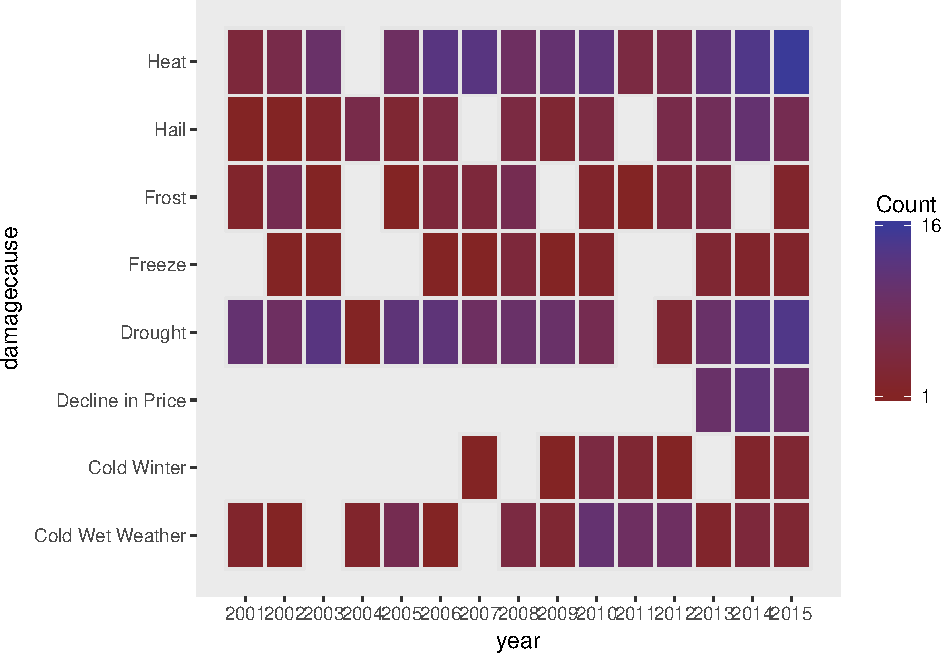
\includegraphics{dmine-mixedmodel-analysis_Phase1_files/figure-latex/unnamed-chunk-21-1.pdf}

IPNW region CHERRIES total insurance loss by damage cause, 2001-2015

2001-2015

damagecause

loss

Excessive Moisture

\$20,569,890

Frost

\$15,459,348

Freeze

\$14,625,022

Decline in Price

\$8,447,020

Cold Wet Weather

\$6,725,206

Heat

\$2,246,093

Hail

\$2,034,613

Other (Snow-Lightning-Etc.)

\$1,876,035

Other

\$1,467,713

Wind/Excess Wind

\$1,402,854

\includegraphics{dmine-mixedmodel-analysis_Phase1_files/figure-latex/unnamed-chunk-22-1.pdf}
\includegraphics{dmine-mixedmodel-analysis_Phase1_files/figure-latex/unnamed-chunk-22-2.pdf}
\includegraphics{dmine-mixedmodel-analysis_Phase1_files/figure-latex/unnamed-chunk-22-3.pdf}
\includegraphics{dmine-mixedmodel-analysis_Phase1_files/figure-latex/unnamed-chunk-22-4.pdf}

\begin{verbatim}
## Error in brewer.pal(11, "YlOrRd"): could not find function "brewer.pal"
\end{verbatim}

\begin{verbatim}
## Error in pal(county_cherries_moisturefrostfreeze$loss): could not find function "pal"
\end{verbatim}

\begin{verbatim}
## Error in getMapData(map): object 'map' not found
\end{verbatim}

\begin{verbatim}
## $interactive
## [1] TRUE
## 
## $draggable
## [1] FALSE
## 
## $keyboard
## [1] TRUE
## 
## $title
## [1] ""
## 
## $alt
## [1] ""
## 
## $zIndexOffset
## [1] 0
## 
## $opacity
## [1] 1
## 
## $riseOnHover
## [1] TRUE
## 
## $riseOffset
## [1] 250
\end{verbatim}

\includegraphics{dmine-mixedmodel-analysis_Phase1_files/figure-latex/unnamed-chunk-22-5.pdf}

\begin{verbatim}
## Error in brewer.pal(11, "YlOrRd"): could not find function "brewer.pal"
\end{verbatim}

\begin{verbatim}
## Error in pal(county_cherries_moisturefrostfreeze2014$loss): could not find function "pal"
\end{verbatim}

\begin{verbatim}
## Error in getMapData(map): object 'map' not found
\end{verbatim}

\begin{verbatim}
## $interactive
## [1] TRUE
## 
## $draggable
## [1] FALSE
## 
## $keyboard
## [1] TRUE
## 
## $title
## [1] ""
## 
## $alt
## [1] ""
## 
## $zIndexOffset
## [1] 0
## 
## $opacity
## [1] 1
## 
## $riseOnHover
## [1] TRUE
## 
## $riseOffset
## [1] 250
\end{verbatim}

\includegraphics{dmine-mixedmodel-analysis_Phase1_files/figure-latex/unnamed-chunk-22-6.pdf}

\begin{verbatim}
## Error in brewer.pal(11, "YlOrRd"): could not find function "brewer.pal"
\end{verbatim}

\begin{verbatim}
## Error in pal(county_cherries_moisturefrostfreeze2015$loss): could not find function "pal"
\end{verbatim}

\begin{verbatim}
## Error in getMapData(map): object 'map' not found
\end{verbatim}

\begin{verbatim}
## $interactive
## [1] TRUE
## 
## $draggable
## [1] FALSE
## 
## $keyboard
## [1] TRUE
## 
## $title
## [1] ""
## 
## $alt
## [1] ""
## 
## $zIndexOffset
## [1] 0
## 
## $opacity
## [1] 1
## 
## $riseOnHover
## [1] TRUE
## 
## $riseOffset
## [1] 250
\end{verbatim}

\includegraphics{dmine-mixedmodel-analysis_Phase1_files/figure-latex/unnamed-chunk-22-7.pdf}
/

\subsubsection{Top Damage Causes for DRY PEAS, 2001-2015 for the Palouse
Region}\label{top-damage-causes-for-dry-peas-2001-2015-for-the-palouse-region}

\includegraphics{dmine-mixedmodel-analysis_Phase1_files/figure-latex/unnamed-chunk-23-1.pdf}

IPNW region DRY PEAS total insurance loss by damage cause, 2001-2015

2001-2015

damagecause

loss

Drought

\$22,635,712

Heat

\$10,399,165

Excessive Moisture

\$8,618,433

Hail

\$5,176,545

Cold Wet Weather

\$2,971,140

Decline in Price

\$2,936,766

Other

\$2,067,635

Wind/Excess Wind

\$1,079,927

Frost

\$924,053

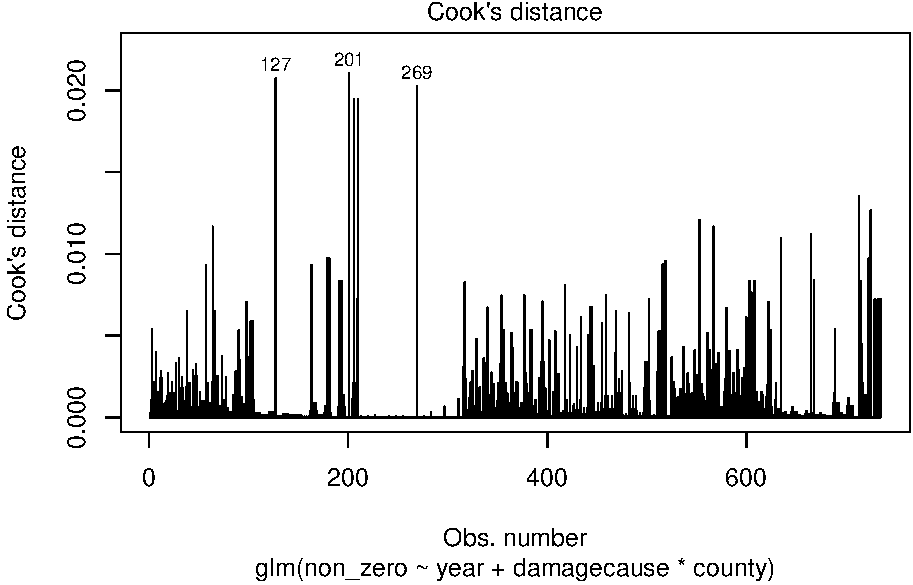
\includegraphics{dmine-mixedmodel-analysis_Phase1_files/figure-latex/unnamed-chunk-24-1.pdf}
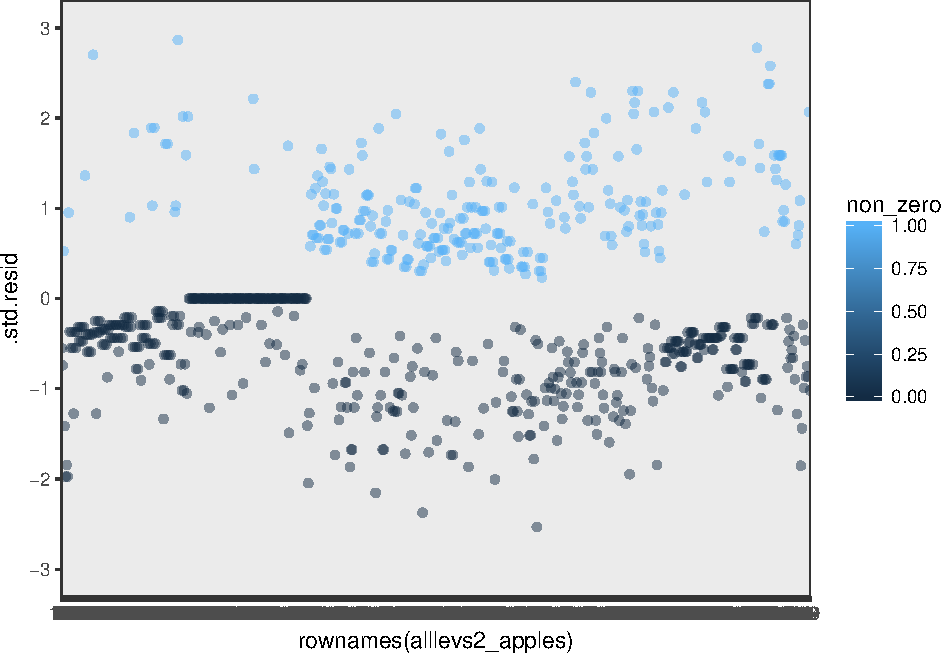
\includegraphics{dmine-mixedmodel-analysis_Phase1_files/figure-latex/unnamed-chunk-24-2.pdf}
\includegraphics{dmine-mixedmodel-analysis_Phase1_files/figure-latex/unnamed-chunk-24-3.pdf}
\includegraphics{dmine-mixedmodel-analysis_Phase1_files/figure-latex/unnamed-chunk-24-4.pdf}
/

\end{document}
